\documentclass[notes]{beamer}       		% compila sia i frame che le note
%\documentclass{beamer}              				% compila solo i frame
%\documentclass[notes=only]{beamer}  	% compila solo le note

% ita language and encoding
\usepackage[utf8]{inputenc}
%\usepackage[italian]{babel}

% formattazione
\usepackage{ragged2e} 							% pacchetto che contiene il comando \justifying
%\apptocmd{\frame}{}{\justifying}{}  	% --> applica la giustificazione a tutti i frame del documento
%\justifying											% --> applica la giustificazione a tutto il documento
\usepackage{hyperref}

% graphics style
\usepackage{graphicx}
\usepackage{xcolor}
\usepackage{shadowtext}

%tabelle
\usepackage{tabularx}
\usepackage{multirow}
\usepackage{booktabs} % aggiunge: \toprule , \midrule e \bottomrule ; stile tabella

%image paths
\graphicspath{	
	{./Images/}
}

% impostazioni base delle slide - tema, colori, caratteri, ... (deic.uab.es/~iblanes/beamer_gallery/)
\mode<presentation>
{
	%\usetheme{CambridgeUS}      	% or try Darmstadt, Madrid, Warsaw, ...
  	\usecolortheme{orchid} 				% for the color box (or try rose ...)
	\usefonttheme{structurebold} 	% or try structureitalicserif, structuresmallcapsserif
}



%% ---------------------------------------------------------------------------------------------------------
% %	CREAZIONE TEMA 

%%    Impostazione dei colori - COLORTHEME 
% (modifica di "beamercolorthemebeaver.sty" in "MiKTeX 2.9/tex/latex/beamer/themes/color" )
\definecolor{darkblue}{RGB}{52,57,176}

\setbeamercolor{section in toc}{fg=black,bg=white}
\setbeamercolor{alerted text}{fg=darkblue!80!gray}
\setbeamercolor*{palette primary}{fg=darkblue!60!black,bg=gray!30!white}
\setbeamercolor*{palette secondary}{fg=darkblue!70!black,bg=gray!15!white}
\setbeamercolor*{palette tertiary}{bg=darkblue!80!black,fg=gray!10!white}
\setbeamercolor*{palette quaternary}{fg=darkblue,bg=gray!5!white}

\setbeamercolor*{sidebar}{fg=darkblue,bg=gray!15!white}

\setbeamercolor*{palette sidebar primary}{fg=darkblue!10!black}
\setbeamercolor*{palette sidebar secondary}{fg=white}
\setbeamercolor*{palette sidebar tertiary}{fg=darkblue!50!black}
\setbeamercolor*{palette sidebar quaternary}{fg=gray!10!white}

%\setbeamercolor*{titlelike}{parent=palette primary}
\setbeamercolor{titlelike}{parent=palette primary,fg=darkblue}
\setbeamercolor{frametitle}{bg=gray!10!white}
\setbeamercolor{frametitle right}{bg=gray!60!white}

\setbeamercolor*{separation line}{}
\setbeamercolor*{fine separation line}{}


%%     Impostazione dei blocchi - INNERTHEME 
% (modifica di "beamerinnerthemerounded.sty" in "MiKTeX 2.9/tex/latex/beamer/themes/inner" )
%\setbeamertemplate{blocks}[rounded]
%\setbeamertemplate{items}[ball]
%\setbeamertemplate{sections/subsections in toc}[ball]
%\setbeamertemplate{title page}[default][colsep=-4bp,rounded=true]
%\setbeamertemplate{part page}[default][colsep=-4bp,rounded=true]


%	%    Impostazione delle intestazioni - OUTERTHEME
% (modifica di "beamerouterthemeinfolines.sty" in "MiKTeX 2.9/tex/latex/beamer/themes/outer" )
\setbeamercolor{institute in head/foot}{parent=palette secondary}
\setbeamercolor{subject in head/foot}{parent=palette tertiary}
\setbeamercolor{title in head/foot}{parent=palette primary}
\setbeamertemplate{footline}
{ 
	\leavevmode%
	\hbox{%
  		% "ht" è lo spazio sopra il carattere partendo dalla base del carattere, "dp"  è lo spazio sotto il carattere partendo sempre dalla base del carattere
  		\begin{beamercolorbox}[wd=.333333\paperwidth,ht=2.5ex,dp=1ex,left,leftskip=4ex]{author in head/foot}%
   			\usebeamerfont{author in head/foot}\insertshortauthor
  		\end{beamercolorbox}%
  		\begin{beamercolorbox}[wd=.333333\paperwidth,ht=2.5ex,dp=1ex,center]{institute in head/foot}%
    		\usebeamerfont{title in head/foot}\insertshortinstitute
 		 \end{beamercolorbox}%
 		 \begin{beamercolorbox}[wd=.333333\paperwidth,ht=2.5ex,dp=1ex,right,rightskip=4ex]{date in head/foot}%
 		 	\usebeamerfont{date in head/foot}\insertshortdate{}\hspace*{2em}\insertframenumber{} / \inserttotalframenumber
 		 \end{beamercolorbox}
 		 }%
 	\vskip0pt%
}
\makeatletter
\setbeamertemplate{headline}
{
  \leavevmode%
  \hbox{%
  \begin{beamercolorbox}[wd=.5\paperwidth,ht=2.8ex,dp=1.35ex,left]{subject in head/foot}	
    \usebeamerfont{section in head/foot}\hspace*{4ex}Complements of Condensed Matter Physics			% --> N.B. Qui c'è l'unica scritta che non usa nessun template tipo \title o \institute
  \end{beamercolorbox}%
  \begin{beamercolorbox}[wd=.5\paperwidth,ht=2.8ex,dp=1.35ex,right]{title in head/foot}%
    \usebeamerfont{subsection in head/foot}\insertshorttitle\hspace*{4ex}
  \end{beamercolorbox}}%
  \vskip0pt%
}
\makeatother

%%    FINE IMPOSTAZIONI TEMA
%% ---------------------------------------------------------------------------------------------------------



% settagio dati principali del file - titolo, autore, ...
\title[Selected concepts of Molecular Dynamics Simulation]{Molecular Dynamics Simulation}
\subtitle{A brief introduction of selected concepts}
\author{Daniele Di Bari}
\institute{University of Perugia}
\date{5th March 2018}
\subject{Complements of Condensed Matter Physics}

% By default the beamer class adds navigation buttons in the bottom right corner. To remove them one can place
\beamertemplatenavigationsymbolsempty

% settaggio prima slide
\setbeamertemplate{title page}
{
	\shadowcolor{white!30!black}
	\vspace{0.75cm}	   
	
	\hbox{
		\begin{beamercolorbox}[wd=.04\textwidth]{white}\end{beamercolorbox}%
  		\begin{beamercolorbox}
  		[wd=.92\textwidth,ht=.115\paperheight,dp=0.2cm,center,rounded=true]{subject in head/foot}%
   			\centering
   			\shadowtext{\textcolor{white}{\textbf{\LARGE \inserttitle}}}
   			
   			\vspace*{0.05cm}
			\shadowtext{\textcolor{white}{\emph{\large \insertsubtitle}}}		
  		\end{beamercolorbox}%
  		
  		
 	}
 	
 	\vspace{0.2cm}
 	
    \begin{center}
  		  		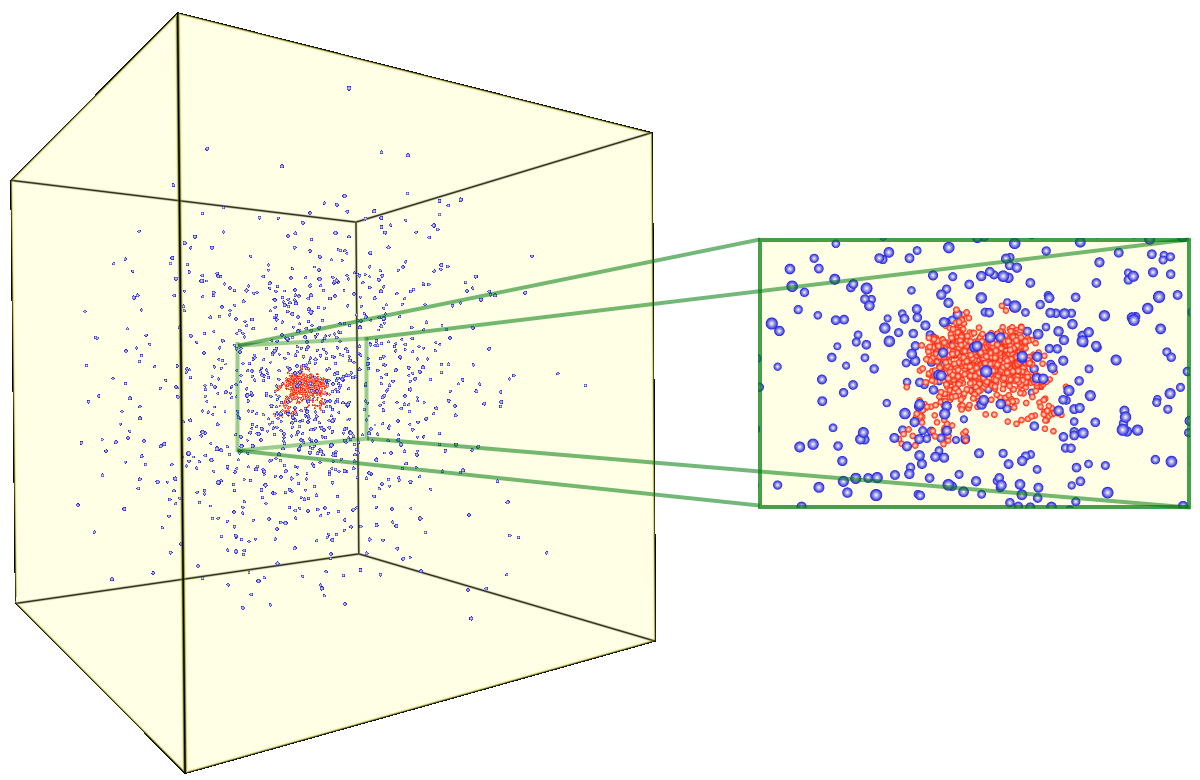
\includegraphics[width=0.8\textwidth,keepaspectratio]{zoom-03.png}
  	\end{center}
%    \begin{colorbox}{darkblue}{ \parbox{0.8\paperwidth}{
%    	\shadowtext{\textcolor{white}{\textbf{\footnotesize{ }}}}
%    	
%    	\vspace{0.2cm}  	
%    	
%    	\shadowtext{\textcolor{white}{\textbf{\LARGE \inserttitle}}}\par
%    	
%    	\vspace{0.1cm}  
%    	
%    	\shadowtext{\textcolor{white}{\emph{\large \insertsubtitle}}}\par
%    	
%    	\vspace{0.2cm}  
%    	}}
%    \end{colorbox} 
%   	
   	\vspace{1.5cm}
	

}
				
% colors
\definecolor{itemred}{RGB}{163,0,0}
\definecolor{itemblue}{RGB}{52,57,176}
\definecolor{notegrey}{RGB}{90,90,90}
\definecolor{titlebgd_grey}{RGB}{242,242,242}
\definecolor{titleframe_red}{RGB}{204,0,0}

% COMANDI
% Formato testo generico in titolpage
\newcommand\titlepagetext[2]{\textcolor{#1}{\footnotesize{\textit{{#2}}}}}
\newcommand\colortextbf[2]{\textcolor{#1}{\textbf{#2}}}
\newcommand\bluetextbf[1]{\textcolor{itemblue}{\textbf{#1}}}
\newcommand\bluetextit[1]{\textcolor{itemblue}{\textit{#1}}}
\newcommand\textitem[2]{\textcolor{itemblue}{\textbf{#1} (\textit{#2})}}

% Testo giustificato
\newenvironment<>{justify}{\justifying{}}

\begin{document}
	% impostare una foto come sfondo del frame: 
	%  \usebackgroundtemplate{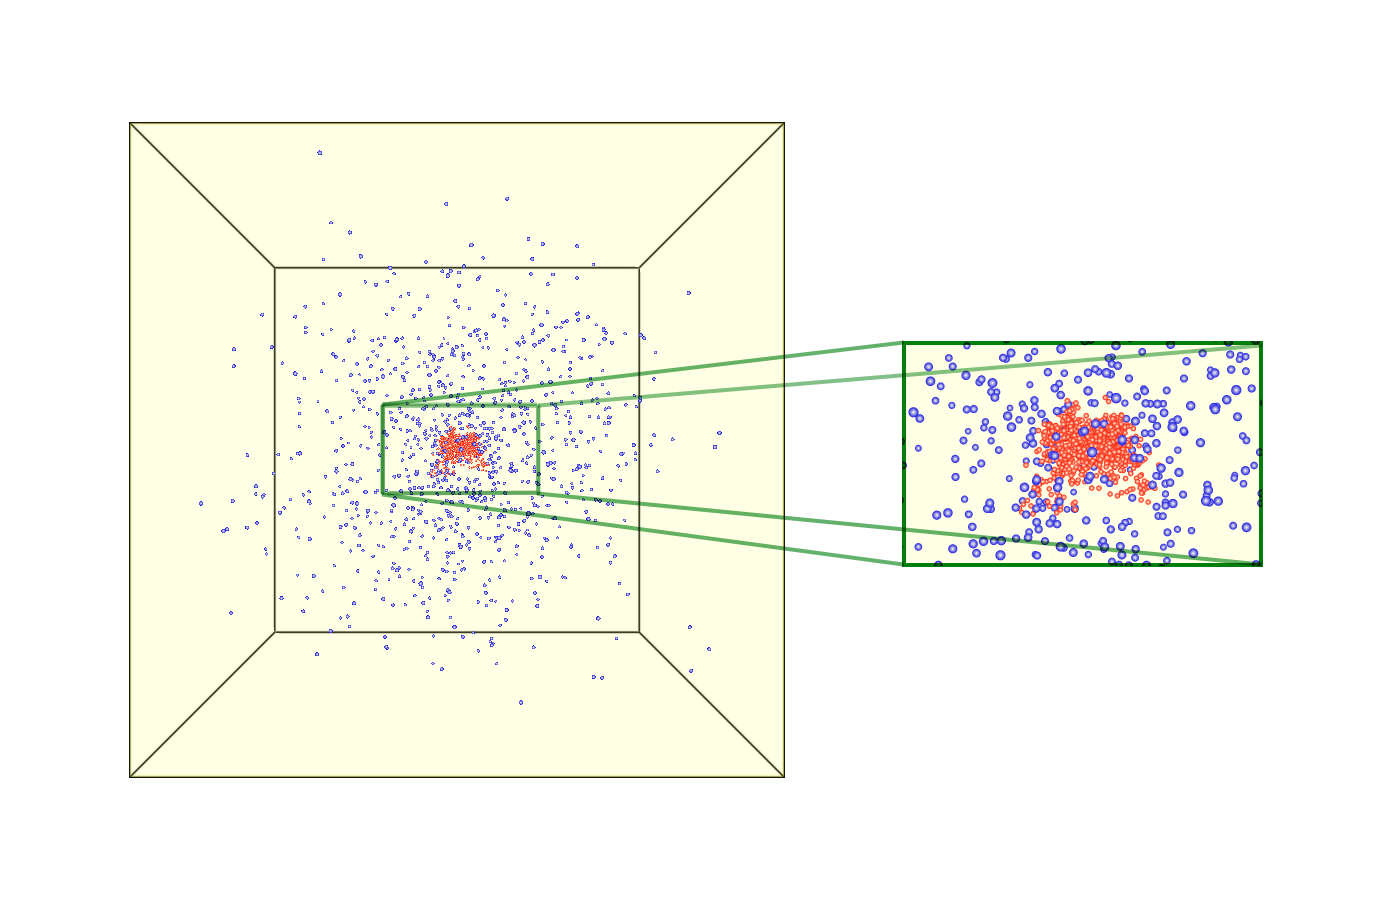
\includegraphics[width=\paperwidth,keepaspectratio]{zoom-01.png}}	
	% 	possibili impostazioni per l'img: width=\paperwidth  --  height=\paperheight  --  keepaspectratio

\begin{frame}\pdfbookmark[2]{Title}{Title}
	\titlepage
\end{frame}

\usebackgroundtemplate{}

\begin{frame}[allowframebreaks]\pdfbookmark[2]{Contents}{Contents}
\frametitle{Table of Contents}
\tableofcontents
\end{frame}

\section{Introduction}
\begin{frame}<presentation:0>[noframenumbering]
	\setbeamertemplate{background}{white}
	\frametitle{Introduction}
	\framesubtitle{The problem of describing complex system}
	\justifying
	
	Few systems in statistical mechanics are exactly soluble, the majority require approximations, but when their complexity increases 
	it becomes difficult even to construct an approximate theory in a reasonable way. 	
	
	\vspace*{0.25cm}
	
	\hspace*{0.3cm}
	\begin{beamercolorbox}[wd=.92\textwidth,center,rounded=true]{institute in head/foot}
   			The more complex and realistic is a system,\\
   			the more difficult and interesting it becomes to describe it.
  	\end{beamercolorbox}%
  	
  	\vspace*{0.2cm}
		
	In this case, an increase in the complexity raises the necessity of having exact results available, both to test existing 
	approximation methods and to point the way towards new approaches. 	
	
	\vspace*{0.2cm}
	
%	\begin{itemize}\justifying
%		\item	\textbf{Computer simulations allow to calculate the essentially exact results for a given model without having to rely on 
%				approximate theories.} 
%	\end{itemize}
	
	\begin{columns}
		\begin{column}{0.1\textwidth}
		\raggedleft
			\hspace*{0.5cm}\textcolor{itemblue}{$\blacktriangleright$}
			
			\vspace*{0.2cm}
			
			\hspace*{0.5cm}\textcolor{itemblue}{$\blacktriangleright$}
		\end{column}
		
		\begin{column}{0.8\textwidth}\justifying
			\textbf{Computer simulations allow to calculate the essentially exact results for a given model without having to rely on 
				approximate theories.} 
		\end{column}
		
		\begin{column}{0.1\textwidth}
			\textcolor{itemblue}{$\blacktriangleleft$}
			
			\vspace*{0.2cm}			
			
			\textcolor{itemblue}{$\blacktriangleleft$}
		\end{column}
	\end{columns}
\end{frame}

\begin{frame}[label=intro-complex_sys]
	\frametitle{Introduction}
	\framesubtitle{The problem of describing complex system}
	\justifying
	
	Few systems in statistical mechanics are exactly soluble, the majority require approximations, but when their complexity increases 
	it becomes difficult even to construct an approximate theory in a reasonable way. 	
	
	\vspace*{0.4cm}
	
	\hspace*{0.3cm}
	\begin{beamercolorbox}[wd=.92\textwidth,center,rounded=true]{institute in head/foot}
   			The more complex and realistic is a system,\\
   			the more difficult and interesting it becomes to describe it.
  	\end{beamercolorbox}%
  	
  	\vspace*{0.35cm}
		
	In this case, an increase in the complexity raises the necessity of having exact results available, both to test existing 
	approximation methods and to point the way towards new approaches. 	
		
%	\begin{itemize}\justifying
%		\item	\textbf{Computer simulations allow to calculate the essentially exact results for a given model without having to rely on 
%				approximate theories.} 
%	\end{itemize}

\end{frame}


\begin{frame}[label=intro-why_use_CS]
	\frametitle{Introduction}
	\framesubtitle{Why to use computer simulations?}
	\justifying
	
	Computer simulations allow to calculate the essentially exact results for a given model without having to rely on approximate theories.
	
	\begin{itemize}\small{\justifying
		\item[$\blacktriangleright$] 	\textbf{TEST THE MODELS:} comparing the results of the simulation with those of a real experiment. 
												If there is disagreement, the model is inadequate - it is necessary to improve on the estimate of the 
												intermolecular interactions.

		\vspace*{0.1cm}												

		\item[$\blacktriangleright$] 	\textbf{TEST THE THEORIES:} comparing the results of the simulation with the predictions of an 
												approximate analytical theory applied to the same model. If there is disagreement, the theory is 
												flawed - the simulation plays the role of the experiment designed to test the theory. 
												This method of screening theories before we apply them to the real world is called a 
												\textit{computer experiment}.

		\vspace*{0.1cm}												
												
		\item[$\blacktriangleright$] 	\textbf{MAKE NUMERICAL PREDICTIONS:} useful to describe a tho- ught experiment and to 
												integrate the macroscopic information with the atomistic level provided by the simulation.
	}\end{itemize}	
	
	%\footnotetext[1]{\justifying The computer simulation plays the role of the experiment designed to test the theory. This method of 
	%screening theories before we apply them to the real world is called a \textit{computer experiment}.}
\end{frame}


\begin{frame}[label=intro-virtual_lab]
	\frametitle{Introduction}
	\framesubtitle{Computer simulations as virtual laboratories}
	\justifying
	
	Computer simulations are similar to a \textbf{virtual laboratory} and, as a consequence, they have several advantages:
	
	\begin{enumerate}\justifying
		\item	Many \textit{virtual experiments can be easily set up} and carried out in succession by simply varying the control 
				parameters
		\item \textit{Extreme\textcolor{white}{y}conditions}, such as high $T$ and $p$, 
				\textit{can\textcolor{white}{y}be created in a simple and considerably safety manner}
		\item	The \textit{time-scales of a system present no impediment} to the simulator thus a wide range of  physical phenomena, 
				from molecular to the galactic, may be studied using computer simulation. 
												%There is no difference between $10^{15} s$ or $10^{-9} s$
	\end{enumerate}

	Technologically useful informations, for systems that may be difficult or even impossible to investigate directly with a real 
	experiment (e.g. nuclear reactors or planetary cores), can be obtained from those type of simulations. 

\end{frame}


\section{Molecular simulations}
\begin{frame}[label=molecular_sim]
	\frametitle{Molecular simulations}
	\framesubtitle{From computer simulations to molecular simulations}
	\justifying
	
	Molecular simulations are computer simulations that study systems from a molecular point of view. 
	\textbf{Starting from an atomistic level, this simulations are used to 
	predict and better understand the properties of complex materials}.\textbf{\footnotemark[1]}
	
	\vspace*{0.25cm}
	
	Molecular simulations provide \underline{a direct route from the microscopic} \underline{details of a system}
	(the masses of the atoms, the	interactions between them, etc.) \underline{to macroscopic properties of experimental interest}
	(the equation of state, transport coefficients and so on).
	
	\vspace*{0.25cm}

	The usefulness of this type of simulations rely on the fact that \textbf{a sample containing a few thousand of particles usually is sufficiently large to simulate the behaviour of a macroscopic system}.
	
	\footnotetext[1]{Even the materials that have not yet been made.}
\end{frame}

%\begin{frame}[label=intro-molecular_sim2]
%	\frametitle{Introduction}
%	\framesubtitle{Molecular simulations - II}
%	\justifying
%	
%	It is clear that molecular simulations have to be able to computing at least the equilibrium properties of a 
%	\textbf{many-body system} and, hopefully, also those of transporting process.
%	
%	\vspace*{0.25cm}
%
%	To perform this type of numerical simulation, it is necessary to \textbf{sample the phase-space} of the system. 
%	When this is done, one has the positions and momenta of all the particles of the system. Thus it is possible to the evaluate the
%	microscopic value of all observables and, eventually, to average them over time or phase-space.
%
%	\vspace*{0.25cm}
%	
%	The downside is that the results of this simulations are only as good as the numerical model and the results can be artificially 
%	biased if the simulation is unable to sample an adequate number of microstates over the time it is allowed to run.
%\end{frame}

\begin{frame}[label=molecular_sim-stat_mech]
	\frametitle{Molecular simulations}
	\framesubtitle{Molecular simulations and statistical mechanics}
	\justifying

	Molecular simulations allow the \textbf{study of the properties of many-particle systems}. 
	However, not all properties can be directly measured in a simulation. Conversely, most of the quantities that can be measured in a 
	simulation do not correspond to properties that are measured in real experiments.
	
	\vspace*{0.25cm}
	
	Actually, \underline{molecular simulations generate information at the micro}-\\
	\underline{scopic level} (atomic and molecular positions, velocities, etc.) 
	and the conversion of this very detailed information into macroscopic terms (pressure, internal energy, etc.) is the field of the 
	statistical mechanics. 
	Thus, the language of \textbf{statistical mechanics is necessary to use these simulations as the numerical counterpart of experiments}.
	
\end{frame}


\subsection{Principal steps}
\begin{frame}[label=molecular_sim-principal_steps]
	\frametitle{Molecular simulations}
	\framesubtitle{The principal steps of molecular simulations}
	\justifying
	
	\vspace*{0.1cm}

	A molecular-scale computer simulation consists of 3 principal steps:
	
	\begin{enumerate}\justifying
		\item Construction of a model
		\item Calculation of molecular trajectories
		\item Analysis of those trajectories to obtain property values
	\end{enumerate}
	
	\vspace*{0.2cm}

	The second step constitutes the \textbf{main feature} of the simulation. In a way that molecular positions $\bold{r}^N$ are computed 
	in this step, thus it is possible to discriminate among the different simulation methods.
	
	\vspace*{0.2cm}
	
	\begin{center}
		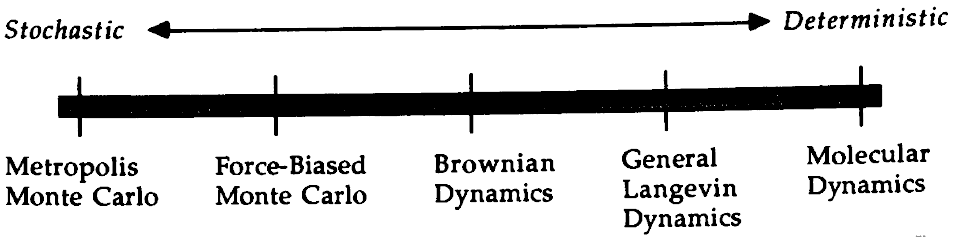
\includegraphics[width=0.7\textwidth]{different_tipes_of_CS.PNG}
	\end{center}
	
\end{frame}


\subsection{Different types}
\begin{frame}[label=molecular_sim-diff_typesd]
	\frametitle{Molecular simulations}
	\framesubtitle{Different types of molecular simulations}
	\justifying
	
	\textbf{Molecular Dynamics -} The positions are obtained by numerically solving differential equations of motion and hence they 
	are connected in time - the positions reveal dynamics of individual molecules as in a motion picture. 
	
	\vspace*{0.3cm}
	
	\textbf{Monte Carlo -} The molecular positions are not temporally related, but are generated stochastically such that a molecular 
	configuration $\bold{r}^N$ depends only on the previous configuration.\footnotemark[1]
	
	\vspace*{0.3cm}
	
	\textbf{Others simulation methods - } The positions are computed from hybrid schemes that use some stochastic features, as 
	in Monte Carlo, and some deterministic features, like in Molecular Dynamics.
	
	\footnotetext[1]{\justifying When the outcome of a random event in a sequence depends only on the outcome of the immediately 
	previous one, the sequence is called: \textit{Markov chain}.}
\end{frame}


\subsubsection{Molecular Dynamics or  Monte Carlo}
\begin{frame}[label=molecular_sim-MCSvsMDS1]
	\frametitle{Molecular simulations}
	\framesubtitle{Molecular Dynamics or  Monte Carlo - I}
	\justifying
	
	The choice between Molecular Dynamics (MD) and Monte Carlo (MC) is largely determined by the phenomenon under investigation.
	
	\begin{itemize}\justifying\small{
		\item \textbf{Monte Carlo is preferable for GAS (}\textit{or other low density systems}\textbf{):}\\
		There can be large energy barriers (of several $k_B T$) which can lead to molecules being trapped in a few low energy 
		conformations in a MD simulation, leading to poor conformational sampling.
		In contrast, the random moves in a MC simulation can easily lead to barrier crossings. 
		
		\vspace*{0.07cm}
		
		\item \textbf{Molecular Dynamics is preferable for LIQUIDS:}\\
		Molecular Collisions exchange energy between them, enabling barrier crossings, improving the ability of MD to sample conformations.
		For a MC simulation, there is a large probability of selecting random moves for which two or more molecules overlap leading to large 
		number of rejected moves and a decrease in efficiency of sampling.\footnote{However, the ability of MC to make unphysical moves, for example to flip a molecule around, can in some cases compensate for this.}
	}\end{itemize}
	
%[Dr S J Clark - http://cmt.dur.ac.uk/sjc/thesis_dlc/node58.html]
\end{frame}


\begin{frame}[label=molecular_sim-MCSvsMDS2]
	\frametitle{Molecular simulations}
	\framesubtitle{Molecular Dynamics or  Monte Carlo - II}
	\justifying
			
	In any cases, there are some situations where only one method is appropriate. In particular:
	
	\vspace*{0.2cm}

	\begin{enumerate}\justifying
		\item	\textbf{Determination of transport properties}, such as viscosity coefficients, is largely only possible using
					\textbf{Molecular Dynamics}, as Monte Carlo lacks an objective definition of time 
					(except in some special cases such as the bond fluctuation model for polymers). 
					
		\vspace*{0.2cm}

		\item	%On the other hand, \textbf{Monte Carlo} can be used for simulations with \textbf{varying particle numbers} 
					%(Grand Canonical Monte Carlo) by adding moves for the creation and destruction of particles.
					Simulations with \textbf{varying particle numbers} that can be made using \textbf{Monte Carlo} methods
					(Grand Canonical Monte Carlo) by adding moves for the creation and destruction of particles.
	\end{enumerate}	 
	
%[Dr S J Clark - http://cmt.dur.ac.uk/sjc/thesis_dlc/node58.html]
\end{frame}
	

\section{Monte Carlo simulation}
\begin{frame}[label=MCS-intro1]
	\frametitle{Monte Carlo simulations}
	\framesubtitle{A summary of Monte Carlo simulations - I}
	\justifying
	
	Monte Carlo simulation is a purely stochastic method typically used to evaluate statistical-mechanical ensemble averages, i.e. 
	multidimensional integrals performed of a $N$-body system. 
	
	\vspace*{0.3cm}
	
	Those integrals are evaluated by accumulating the integrand at random generated values of the independent variables that define 
	a configuration of the system (usually the position $ \bold{r}^N$, possibly also the volume of the system or the number of particles 
	that it contains). 
	
	\vspace*{0.3cm}
	
	\textbf{The particle momenta do not enter the calculation, there is no time scale involved, and the order in which the 
	configurations occur has no special significance. The method is therefore limited to the calculation of static properties.}
	
\end{frame}


\begin{frame}[label=MCS-intro2]
	\frametitle{Monte Carlo simulations}
	\framesubtitle{A summary of Monte Carlo simulations - II}
	\justifying
	
	\vspace*{-0.2cm}
	\textbf{Not all configurations that are generated are accepted.} 
	The choice of rejecting or not a new configuration is made in such a way that, asymptotically, the configuration space is sampled 
	according to the probability density corresponding to a particular ensemble.\footnotemark[1] 
	
	For example, in the canonical ensemble the average of a microscopic variable $A ( \bold{r}^N )$ is:
	\begin{equation}\label{eq:can_ens:avg_val}
		\left< A \right> = \frac{1}{Z}	\int \cdots \int \, A ( \bold{r}^N ) \; e^{ -\beta \, U( \bold{r}^N)} \; d\bold{r}_1 \cdots d\bold{r}_N
	\end{equation}
	Due to $e^{ -\beta \, U( \bold{r}^N)}$, some configurations contribute largely to the integral while others do it less. 
	Thus, \textbf{it is necessary to bias the sampling in favour of those configurations most likely to occur}.
	
	\footnotetext[1]{\justifying In general, configurations that go against at least one of the system's constrains,  
	e.g. due to an overlap of two hard-spheres, have to be rejected.}

\end{frame}


\subsection{Metropolis method}
\begin{frame}[label=MCS-Metropolis1]
	\frametitle{Monte Carlo simulations}
	\framesubtitle{A summary of the Monte Carlo simulations: Metropolis method - I}
	\justifying	
	
	\vspace*{0.2cm}
	
	The Metropolis method used in Monte Carlo simulations involves the following main steps:
	
	\begin{columns}
		\begin{column}{0.00\textwidth}\end{column}
		
		\begin{column}{0.68\textwidth}\justifying
			\begin{enumerate}\justifying
				\item	\textbf{Starting from a configuration} $m$. If this is the 1st step, initializing the positions and computing the 
				potential energy.
				\item \textbf{Generating a trial configuration} $n\,$ by selecting a particle $i\,$ at random and giving it a small, random
						displacement, $\bold{r}^n_i \rightarrow \bold{r}^n_i + \Delta\bold{r}$, where $\Delta\bold{r}$ is chosen uniformly 
						within prescribed limits.
			\end{enumerate}
		\end{column}
		
		\begin{column}{0.32\textwidth}
			\centering	
			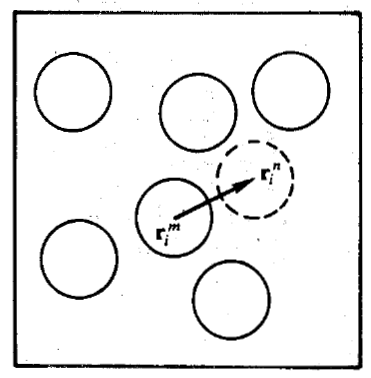
\includegraphics[width=\textwidth]{Metropolis.PNG}
		\end{column}	
		
		\begin{column}{0.00\textwidth}\end{column}
	\end{columns}	
	
	\begin{columns}
		\begin{column}{0.705\textwidth}\end{column}
		
		\begin{column}{0.35\textwidth}
			\centering	
			
			\vspace*{-0.3cm}
			\scriptsize{\bluetextbf{	Schematic view of
											a random displacement
											of the $i$-particle from $\bold{r}^m_i$ to $\bold{r}^n_i$}}					
		\end{column}	
		
		\begin{column}{0.00\textwidth}\end{column}
	\end{columns}	
	
\end{frame}


\begin{frame}[label=MCS-Metropolis2]
	\frametitle{Monte Carlo simulations}
	\framesubtitle{A summary of the Monte Carlo simulations: Metropolis method - II}
	\justifying
	
	\begin{enumerate}\justifying
		\item[3.] \textbf{Verifying} whether \textbf{the trial configuration} must be rejected:
					\begin{itemize}\justifying
						\item \bluetextbf{yes:} count the old configuration $n$ as the new configuration $m$ and repeat the process from 
								step 1
						\item \bluetextbf{not:} compute the new potential energy $U_n$ and accept the proposed configuration with the 
								following:
								
								\vspace*{-0.5cm}
								\begin{equation*}
									\hspace*{0.35cm}\begin{cases}
									\text{if } U_n < U_m \Longrightarrow \text{accept with probability} = 1\\
									\text{if } U_n > U_m \Longrightarrow \text{accept with probability} \propto  e^{ -\beta \, (U_n\, - U_m)} 
									\end{cases}	
								\end{equation*} 
					\end{itemize}
		\item[4.] \textbf{Evaluating property integrands}, such as $A(\bold{r}^N)$ in \eqref{eq:can_ens:avg_val}, and accumulating them in 
					running sums
		\item[5.] \textbf{Iterate the entire process} until at least a few million of configurations have been made to obtain an adequate 
					statistical error in the average values
	\end{enumerate}
	
\end{frame}


\section{Molecular Dynamics Simulations}
\subsection{Classical Approximation}
\begin{frame}[label=MDS-Clas_approx1]
	\frametitle{Molecular Dynamics Simulations}
	\framesubtitle{Computing the internal motion of classical many-body systems}
	\justifying

	Molecular Dynamics simulations compute the motions of individual molecules for a classical many-body system in order to describe the 
	equilibrium and transport properties of solids, liquids and gasses.	
	
	\vspace*{0.2cm}
	
	\hspace*{0.25cm}
	\begin{beamercolorbox}[wd=.93\textwidth,center,rounded=true]{institute in head/foot}
	\small{
   			Although this modelling of the matter at the microscopic level
   			%(\textit{based on a comprehensive description of the constituent particle})\\
   			must be, in principle, based on quantum mechanics,\\
   			\hspace*{0.1cm}\textbf{Molecular Dynamics generally adopts a classical point of view}
   	}
  	\end{beamercolorbox}%
	
	\vspace*{0.2cm}
	
	In this context, the word classical means that the nuclear motion of the constituent particles obeys the laws of classical mechanics 
	(the motion is described by the second Newton's law). 
	
	\vspace*{0.2cm}
		
	This is an \textbf{excellent approximation for a wide range of materials}.	
\end{frame}


\begin{frame}[label=MDS-Clas_approx2]
	\frametitle{Molecular Dynamics Simulations}
	\framesubtitle{Classical approximation}
	\justifying
	
	\vspace*{-0.25cm}
	
	\begin{block}{\small{Neither relativistic nor quantum effects are considered}}\justifying\small{
		\textbf{Special relativity} does not allow information to travel faster than light; Molecular Dynamics simulations assume forces with 
		an infinite speed of propagation. 
	
		\textbf{Quantum mechanics} has at its base the uncertainty principle; Molecular Dynamics requires, and provides, complete 
		information about position and momentum at all times.
	}\end{block}

	\vspace*{0.05cm}
	
	In practice, the phenomena studied by Molecular Dynamics simulation are those where relativistic effects are not observed and 
	quantum effects can, if necessary, be incorporated as semi-classical corrections derived from quantum theory.\footnotemark[1]

	\footnotetext[1]{\justifying For example, dealing with very light atoms or molecules (e.g. He, $\text{H}_2$, $\text{D}_2$) or with 
	vibrational motions whose characteristic frequency, translated in energy, is comparable or larger than $k_B T$, quantum effects became 
	not negligible.}
\end{frame}


\subsection{Microcanonical ensamble}
\begin{frame}[label=MDS-ensemble1]
	\frametitle{Molecular Dynamics Simulations}
	\framesubtitle{Connection between microcanonical ensemble and Hamiltonian mechanics}
	\justifying
	
	The microcanonical ensemble consists of all microscopic states $ ( \bold{q}^N, \bold{p}^N )$ on the constant energy hypersurface 
	$H ( \bold{q}^N, \bold{p}^N ) = E$. 
	
	\vspace*{0.15cm}
	
	In classical Hamiltonian mechanics the equations of motion conserve the total energy: 
	$dH/dt = 0 \Rightarrow H ( \bold{q}^N, \bold{p}^N ) = const$.
	
	\vspace*{0.15cm}
	
	This suggests a \textbf{connection between the microcanonical ensemble and classical Hamiltonian mechanics}. 
	
	\vspace*{0.15cm}
	
	Indeed, for a system that evolves according to Hamilton's equations of motion:
	\begin{equation*}
		\dot{\bold{q}}_i = \frac{\partial H}{\partial \bold{p}_i} \quad \quad \dot{\bold{p}}_i = - \frac{\partial H}{\partial \bold{q}_i}
	\end{equation*}
	
	a trajectory computed with these equations will generate microscopic configurations belonging to the microcanonical ensemble with 
	the constant energy $E$.

%	\begin{block}{\small{A consequence of this connection}}\justifying
%	\small{
%		Imagine a system that evolves according to Hamilton's equations of motion:
%		\begin{equation*}
%			\dot{\bold{q}}_i = \frac{\partial H}{\partial \bold{p}_i} \quad \quad \dot{\bold{p}}_i = - \frac{\partial H}{\partial \bold{q}_i}
%		\end{equation*}
%		
%		Since the equations of motion conserve the Hamiltonian $H ( \bold{q}^N, \bold{p}^N )$, a trajectory computed with these 
%		equations will generate microscopic configurations belonging to a microcanonical ensemble with energy $E$.
%	}	
%	\end{block}
%	

\end{frame}


\begin{frame}[label=MDS-ensemble2]
	\frametitle{Molecular Dynamics Simulations}
	\framesubtitle{Generate a microcanonical ensemble}
	\justifying
	
	\vspace*{-0.15cm}

	\begin{columns}
		\begin{column}{0.02\textwidth}\end{column}
		
		\begin{column}{0.46\textwidth}\justifying
			If after a long time a system with energy $E$ is able to visit  practically all the configurations on the constant energy hypersurface, 
			the dynamical evolution of this system can be used to generate a microcanonical ensemble.\footnotemark[1]
		\end{column}
		
		\begin{column}{0.5\textwidth}
			\centering	
			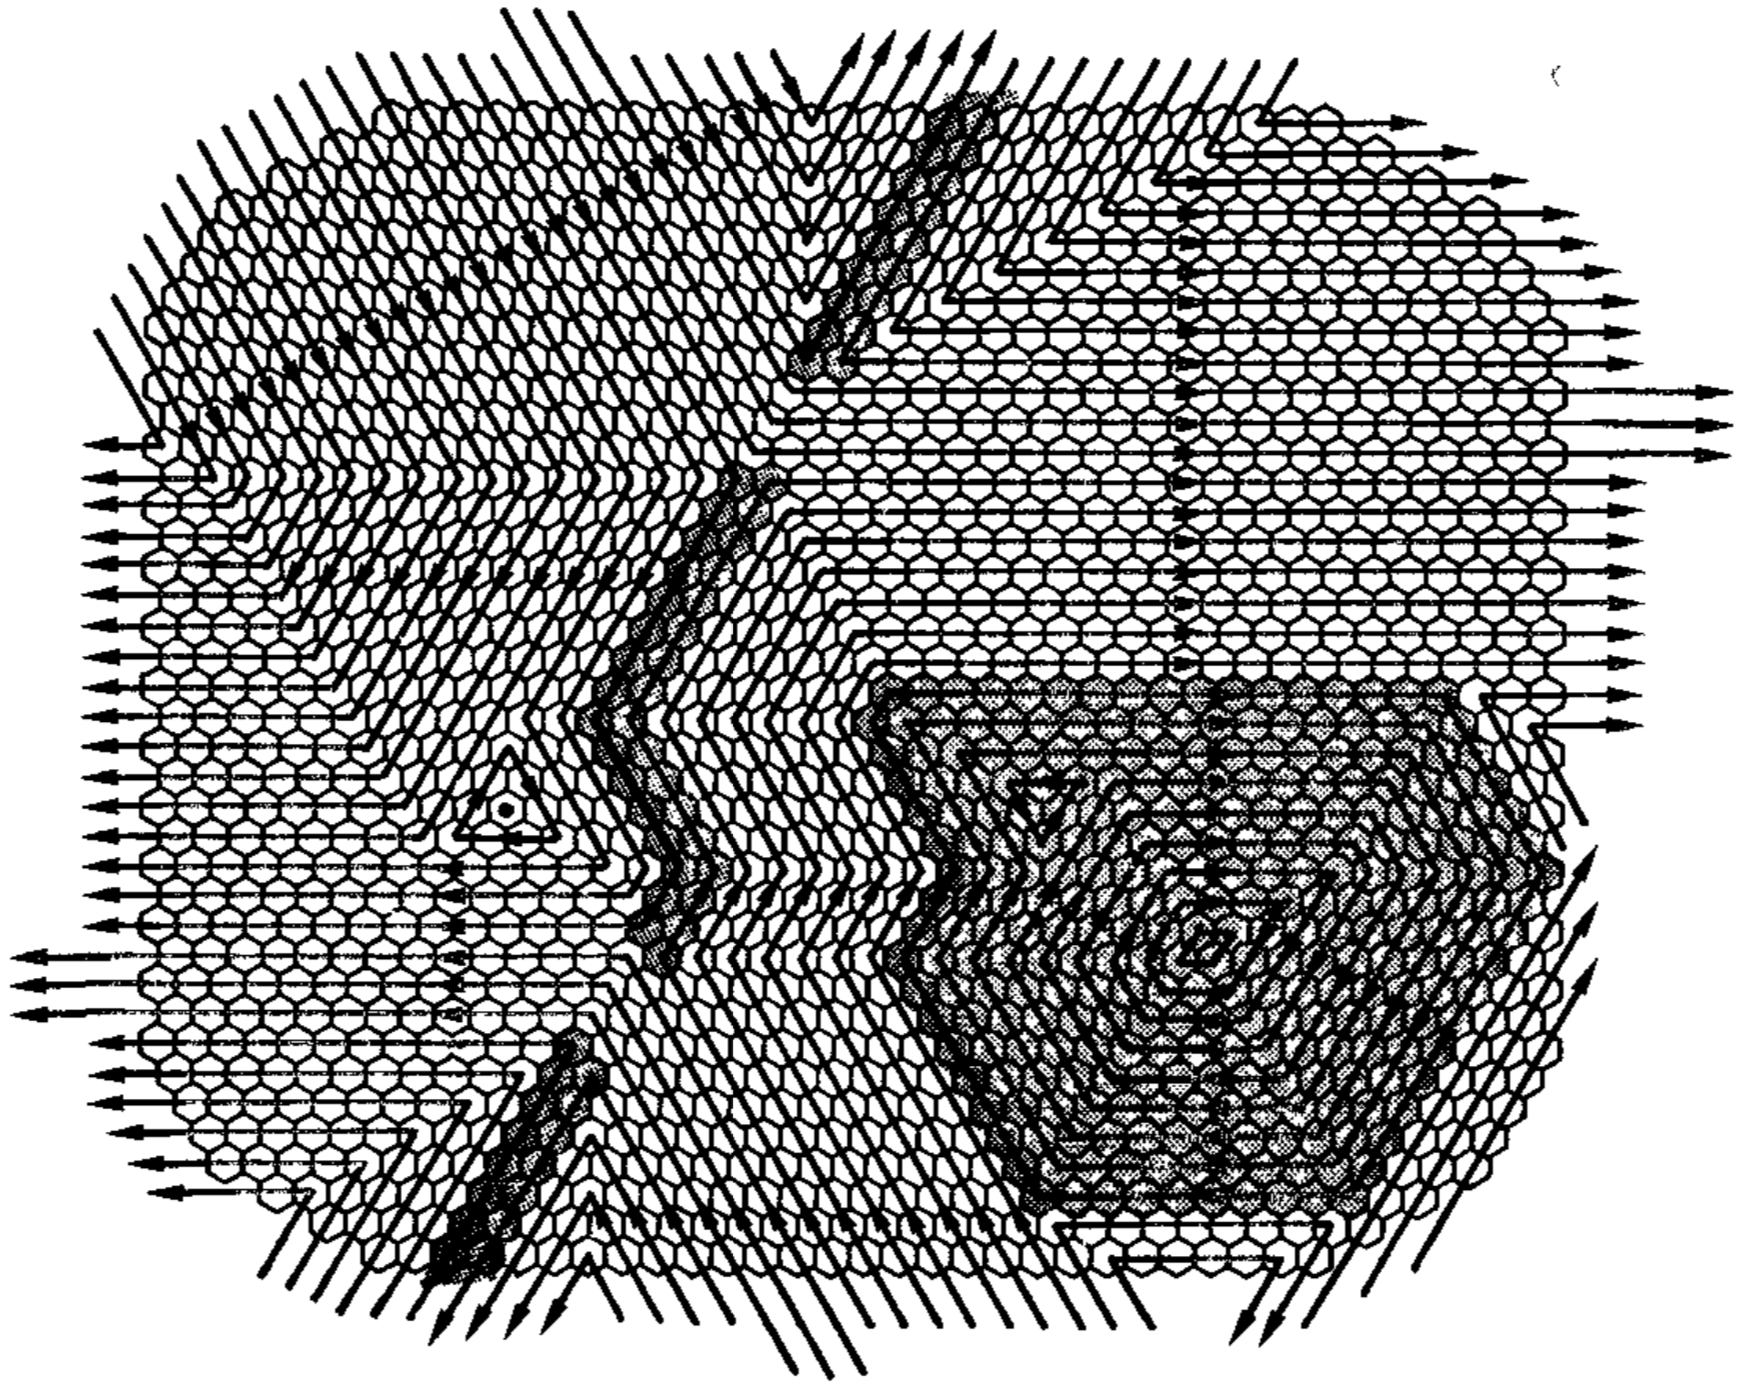
\includegraphics[width=\textwidth]{phase_space.png}
		\end{column}	
		
		\begin{column}{0.02\textwidth}\end{column}
	\end{columns}	
	
	\vspace*{0.2cm}
	
	In general \underline{this dynamical approach}, that is at the basis of MD simulations, 
	\underline{provides a powerful method for generating an ensemble and} \underline{its averages}. 
	Thus MD simulation has evolved into one of the most widely used techniques for solving statistical mechanical problems.

	\footnotetext[1]{A system that has this property is said to be \textit{ergodic}.}
\end{frame}


\begin{frame}[label=MDS-ensemble3]
	\frametitle{Molecular Dynamics Simulations}
	\framesubtitle{Microcanonical phase space averages}
	\justifying
	
	Given an ergodic trajectory, microcanonical phase space averages can be replaced by time averages over the trajectory according to:
	
	\vspace*{-0.1cm}
	
	\begin{equation*}
		\left< A \right> \equiv \frac{\int dx \, A(x) \delta(H ( x ) - E)}{\int dx \, \delta(H ( x ) - E)} = \lim_{\tau \rightarrow \infty} \frac{1}{\tau} \int_0^\tau dt \, A(x_t) \equiv \bar{A}
	\end{equation*}
	
	\vspace*{0.2cm}
	
	discretized for molecular dynamics simulations as\footnotemark[1]:

	\vspace*{-0.2cm}
	
	\begin{equation*}
		\left< A \right> = \frac{1}{M} \sum_{n =1}^M A(x_{n \, \Delta t})
	\end{equation*}
	
	\footnotetext[1]{\justifying{Discretization derive from the fact that the equations of motion are solved numerically using some numerical integrators that generate phase space vectors at discrete times that are multiples of a fundamental time discretization parameter $\Delta t$, known as \textit{the time step}. Starting from $x_0$, the vectors $x_{n \, \Delta t}$ (where $n = 0, \cdots , M$) are generated by applying the integrator iteratively.}}
	
\end{frame}


\subsection{Numerical integrators}
\begin{frame}[label=MDS-mainAsp]
	\frametitle{Molecular Dynamics Simulations}
	\framesubtitle{Main aspects of the calculation}
	\justifying
	
	There are three main aspects for a molecular dynamics calculation: 
	
	\begin{enumerate}\justifying
		\item \textbf{The model} describing the interparticle interactions
		\item \textbf{The calculation of energies and forces} from the model, which should be done accurately and efficiently
		\item \textbf{The numerical integrator employed}, i.e. the algorithm used to integrate the equations of motion
	\end{enumerate}	
	
	Each of these aspects can strongly influence the quality of the calculation and its ability to sample a sufficient number of microstates to 
	obtain reliable averages. 
	
	The present work focuses on the problem of devising a numerical integrator for the equations of motion.

\end{frame}

\subsubsection{Criteria for a good numerical integrator}
\begin{frame}[label=MDS-intCriteria1]
	\frametitle{Molecular Dynamics Simulations}
	\framesubtitle{Criteria for a good numerical integrator - I}
	\justifying
	
	\vspace*{-0.1cm}
	A suitable MD program requires a good algorithm to integrate the equations of motion.	
	In this sense, \textbf{the choice of the numerical integrator employed is crucial}. 
	However, although it is easy to recognize a bad integrator, it is not obvious which criteria a good integrator should satisfy. 
	Indeed there are some points to consider.
	
	\begin{itemize}\justifying
		\item	\bluetextbf{Speed is not very relevant} because, usually, the fraction of time spent on integrating the equations of motion is small 
				compared to computing the interactions.
		
		\item	\bluetextbf{Accuracy for large $\Delta t$ is more important}: the bigger is the $\Delta t$ used, the fewer are evaluations of the 
				forces needed. Hence, it is useful to employ a sophisticated algorithm that allows the use of a long $\Delta t$.\footnotemark[1]
	\end{itemize}
	
	\footnotetext[1]{\justifying Actually some algorithms allow the use of large $\Delta t$, storing information on increasingly higher-order derivatives of the particle coordinates. They require more memory storage, but typically this is not a serious drawback.}
	
\end{frame}

\begin{frame}[label=MDS-intCriteria2]
	\frametitle{Molecular Dynamics Simulations}
	\framesubtitle{Criteria for a good numerical integrator - II}
	\justifying
	
	\begin{itemize}\justifying
		\item	\bluetextbf{Energy conservation is an important criterion.}
				The sophisticated higher-order algorithms tend to have very good energy conservation for short times 
				(i.e., during a few $\Delta t$).
				Nevertheless, they often have the undesirable feature that the overall energy drifts for long times. In contrast, simpler algorithms 
				tend to have only moderate short-term energy conservation but little long-term drift.
		
		\item	\bluetextbf{Time reversibility:} Since the equations of motion are time reversible, so should be the numerical integrator employed. 
				In fact, many algorithms are not time reversible - future and past phase space coordinates do not play a symmetric 
				role.\footnotemark[1]
	\end{itemize}
	
	\footnotetext[1]{\justifying For instance the predictor-corrector schemes and many of the schemes used to deal with constraints.}
	%However, at the moment, there are not algorithms that are able to accurately predicts the trajectory of all particles for both short and long times.
\end{frame}

\begin{frame}[label=MDS-intCriteria3]
	\frametitle{Molecular Dynamics Simulations}
	\framesubtitle{Criteria for a good numerical integrator - III}
	\justifying
	
	The last two criteria are actually related, indeed Hamiltonian dynamics, that is symmetric in time, leaves the magnitude of any volume 
	element in phase space unchanged. 
	However, many numerical integrator, in particular those that are not time reversible, do not reproduce this area-preserving 
	property and this is not compatible with energy conservation.
	
	Therefore, it is plausible that non-reversible algorithms will have serious long-term energy drift problems.
	However, this does not mean that the reversibility alone is sufficient to guarantee the absence of such energy drift. 
%	Actually this property is at least compatible	with it. 	

	\vspace*{0.2cm}
	
	\hspace*{0.25cm}
	\begin{beamercolorbox}[wd=.93\textwidth,center,rounded=true]{institute in head/foot}
	\small{
   			The conservation of volume elements in phase space is a\\
   			fundamental property for a numerical integrator to avoid\\
   			significant	drift in the total energy with time.
   	}
  	\end{beamercolorbox}%
\end{frame}


\subsubsection{Finite-difference method}
\begin{frame}[label=MDS-FDM1]
	\frametitle{Molecular Dynamics Simulations}
	\framesubtitle{Finite-difference method}
	\justifying
	There are several distinct approaches to the formulation of computer methods for solving differential equations. 
	One of the most used in the molecular dynamics simulations is:
	
	\begin{block}{The Finite-Difference Method - FDM}\justifying
		The central idea of this method is to \textbf{approximate the derivatives by differences} and thereby reduce differential equations to
		difference equations.
		
		\begin{itemize}\justifying
			\item	An \textit{analytical} problem becomes an \textit{algebraic} one.
			\item	A problem with an \textit{infinite degree of freedom} is replaced by one with a \textit{finite degree of freedom}.
			\item	A \textit{continuous} problem goes over to a \textit{discrete} one.
		\end{itemize}
	\end{block}

\end{frame}

\begin{frame}[label=MDS-FDM2]
	\frametitle{Molecular Dynamics Simulations}
	\framesubtitle{Finite difference method - A simple example I}
	\justifying
	To introduce this argument, it is useful to start by looking at the two Taylor expansions of $f(x)$:
	\begin{equation}\label{eq:taylor}
		f(x \pm \Delta x) = f(x) \pm f'(x) \cdot \Delta x + \frac{1}{2} f''(x) \cdot \Delta x^2 + O(\Delta x^3)
	\end{equation}
	
%	The higher order terms represented by $O(\Delta x^3)$ become less important as $\Delta x$ becomes smaller. 
	From this equations it is possible to obtain two first approximations for the derivative of $f(x)$:
	\begin{align*}
		f'(x) &= \frac{f(x + \Delta x) - f(x)}{\Delta x} + O(\Delta x) = f'_F(x) + O(\Delta x)\\
		f'(x) &= \frac{f(x) - f(x - \Delta x)}{\Delta x} + O(\Delta x) = f'_B(x) + O(\Delta x)
	\end{align*}
	
	where $f'_F(x)$ and $f'_B(x)$ are the \textbf{forward and backward differences} that both involve approximation of order $O(\Delta x)$.
\end{frame}

\begin{frame}[label=MDS-FDM3]
	\frametitle{Molecular Dynamics Simulations}
	\framesubtitle{Finite difference method - A simple example II}
	\justifying
	Subtracting the two expansions in \eqref{eq:taylor}, yields:
	\begin{equation*}
		f'(x) = \frac{f(x + \Delta x) - f(x - \Delta x)}{2 \Delta x} + O(\Delta x^2) = f'_C(x) + O(\Delta x^2)
	\end{equation*}
	
	where  $f'_C(x)$ is the \textbf{central difference} that involve an approximation of order $O(\Delta x^2)$ and thus, for small $\Delta x$, it is 
	more accurate than $f'_F(x)$ and $f'_B(x)$. 
	
	\vspace*{0.4cm}
	
	Considering $f(t)$ such as the position $\bold{r}$ of a particle at the time $t$, this result can be used to evaluate the velocity of that 
	particle: 
	\begin{equation*}
		\bold{v}(t) \approx \frac{\bold{r}(t + \Delta t) - \bold{r}(t - \Delta t)}{2 \Delta t}
	\end{equation*}
\end{frame}


\begin{frame}[label=MDS-verlet1]
	\frametitle{Molecular Dynamics Simulations}
	\framesubtitle{The Verlet integrator - I}
	\justifying
	
	Let the position of particle $i$ be $\bold{r}_i(t)$. To derive the Verlet algorithm, the position at times $t + \Delta t$ is expressed in terms of 
	its position, velocity and acceleration at time $t$ according to:
	\begin{equation*}
		\bold{r}_i(t + \Delta t) = \bold{r}_i(t) + \dot{\bold{r}}_i(t) \, \Delta t + \frac{\ddot{\bold{r}}_i(t)}{2} \, \Delta t^2 + \frac{\dddot{\bold{r}}_i(t)}{3!} \, \Delta t^3 + O(\Delta t^4)
	\end{equation*}
	
	A velocity-independent scheme can be obtained by writing a similar expansion for $\bold{r}_i(t + \Delta t)$:
	\begin{equation*}
		\bold{r}_i(t - \Delta t) = \bold{r}_i(t) - \dot{\bold{r}}_i(t) \, \Delta t + \frac{\ddot{\bold{r}}_i(t)}{2} \, \Delta t^2 - \frac{\dddot{\bold{r}}_i(t)}{3!} \, \Delta t^3 + O(\Delta t^4)
	\end{equation*}
	
	Adding these two equations, one obtains:
	\begin{equation*}
		\bold{r}_i(t + \Delta t) = 2 \, \bold{r}_i(t) -  \bold{r}_i(t - \Delta t) + \frac{\ddot{\bold{r}}_i(t)}{2} \, \Delta t^2 + O(\Delta t^4)
	\end{equation*}
\end{frame}

\begin{frame}[label=MDS-verlet2]
	\frametitle{Molecular Dynamics Simulations}
	\framesubtitle{The Verlet integrator - II}
	\justifying
	
	Using the Newton's second law, $\ddot{\bold{r}}_i(t) = \bold{F}_i(t) / m_i$, yields:
	\begin{equation*}
		\bold{r}_i(t + \Delta t) = 2 \, \bold{r}_i(t) -  \bold{r}_i(t - \Delta t) + \frac{\bold{F}_i(t)}{2 \, m_i} \, \Delta t^2 + O(\Delta t^4)
	\end{equation*}
	
	Dropping the 	all terms of the order $O(\Delta t^4)$, one obtains the numerical integrator known as the \textbf{Verlet algorithm}:
	\begin{equation*}
		\bold{r}^{verl}_i(t + \Delta t) = 2 \, \bold{r}_i(t) -  \bold{r}_i(t - \Delta t) + \frac{\bold{F}_i(t)}{2 \, m_i} \, \Delta t^2
	\end{equation*}
	
	This algorithm is not only one of the simplest, but also usually one of the best.
\end{frame}

\begin{frame}
	\frametitle{Molecular Dynamics Simulations}
	\framesubtitle{Finite difference method - Errors}
	\justifying
	
	The numerical integrator employed in MD simulation generates the trajectory of the system in the phase space, allowing in this way to 
	measure the properties of interest deriving from that trajectory.
	
	However, in generating trajectories, uncertainties arise from the finite-difference method used (truncation error) and from the way it is 
	implemented (round-off error). Therefore, it is important to study not merely the FDM per se, rather the broader problem of how those 
	methods can affect the reliability of simulation results.
	
	The terms truncation and round-off refer to sources of errors; however, it should be considered not only what causes errors but also how 
	errors propagate - whether they grow as the simulations proceeds. This is the issue of algorithmic stability.
\end{frame}

\begin{frame}
	\frametitle{Molecular Dynamics Simulations}
	\framesubtitle{Finite difference method - Errors}
	\justifying
	
	Molecular dynamics involves nonlinear ordinary differential equations, so analytical stability analysis cannot be used. Instead, it may do an approximate analysis by linearizing the differential equations or it may attack the stability problem using the method of Lyapunov. Both strategies are cumbersome when applied to the equations of motion used in molecular dynamics, thus what it is usually done for simple simulations is a numerical analysis using trial values for the time step. That is, through a series of short test runs, it is possible to identify the critical step $\Delta t$ at which the algorithm becomes unstable and then choose a smaller operational value that establishes conservation of energy. 
\end{frame}



\begin{frame}
	\frametitle{Introduction}
	\framesubtitle{What is a MD Simulation?}
	\justifying
	Molecular dynamics simulations compute the motions of individual molecules in models of solids, liquids and gasses. The key idea is motion, which describes how positions, velocities and orientations change with time. In effect, molecular dynamics constitutes a motion picture that follows molecules as they dart to and fro, twisting, turning, colliding with one another and, perhaps, colliding with their container.
\end{frame}

\begin{frame}
	\frametitle{Introduction}
	\framesubtitle{What is a MD Simulation?}
	\justifying
Historically, the choice
of algorithm was often determined in large part by the amount of computer
memory needed, i.e. the number of variables that needed to be kept track of.
Given the large memories available today, this concern has been largely
ameliorated. Two features that we do want to mention here which were
introduced to make molecular dynamics simulations faster are potential ``cutoffs''
and ``neighbor lists''. (These labor saving devices can also be used for
Monte Carlo simulations of systems with continuous symmetry.) As the
particles move, the forces acting on them change and need to be continuously
recomputed. A way to speed up the calculation with only a modest
reduction in accuracy is to cut off the interaction at some suitable range and
then make a list of all neighbors which are within some slightly larger radius.
As time progresses, only the forces caused by neighbors within the ``cutoff
radius’ need to be recomputed, and for large systems the reduction in effort
can be substantial. (The list includes neighbors which are initially beyond
the cutoff but which are near enough that they might enter the ``interacting
region'' within the number of time steps, typically 10–20 which elapse before
the list is updated.) With the advent of parallel computers, molecular
dynamics algorithms have been devised that will distribute the system
over multiple processors and allow treatment of quite large numbers of
particles. One major constraint which remains is the limitation in maximum
integration time and algorithmic improvement in this area is an important
challenge for the future.
\end{frame}

\section{Bibliography}
\begin{frame}[allowframebreaks]
	\frametitle{Sources}
	\justifying
		
	\bluetextbf{Books on Molecular Dynamics Simulation}
	
	\begin{thebibliography}{99}
	\setbeamertemplate{bibliography item}[text]
	\scriptsize{\justifying
	\bibitem{books:Allen}
	Allen, M., \& Tildesley, D. (1987). \textit{Computer Simulation of Liquids}. Oxford, England, Clarendon Press.

	\bibitem{books:Frenkel}
	Frenkel, D., \& Smit, B. (2012). \textit{Understanding molecular simulation: from algorithms to applications}. 
	San Diego, Calif.: Academic Press.	
	
	\bibitem{books:Haile}
	Haile, J. M. (1992). \textit{Molecular dynamics simulation: elementary methods}. New York u.a.: Wiley.
	
	\bibitem{books:Hansen}
	Hansen, J. P., \& McDonald, I. R. (2014). \textit{Theory of simple liquids: with applications to soft matter}. Amsterdam: Elsevier. 
	
	\bibitem{books:Tuckerman}
	Tuckerman, M. E. (2010). \textit{Statistical Mechanics: Theory and Molecular Simulation}. New York, United States: 
	Oxford University Press. 
	
	
	\bibitem{site:Cheung}
	Cheung, D. L. (2002). \textit{Structures and Properties of Liquid Crystals and Related Molecules from Computer Simulation} 
	 (Ph.D. Thesis).\\Retrieved from: \url{http://cmt.dur.ac.uk/sjc/thesis_dlc/}
	 
	 \justifying
	 \bibitem{}
	 Lynch, P. (2005–2006). \textit{Numerical Weather Prediction}. Lecture presented at Course of Meteorology \& Climate Centre in University College Dublin. \\Retrieved from: \url{http://www.atmos.umd.edu/~ekalnay/syllabi/AOSC614/NWP-CH03-1-2.pdf} 
	 }
	
	\end{thebibliography}
\end{frame}



\end{document}
